\chapter{Lực tương tác giữa các dây dẫn thẳng dài đặt song song có dòng điện chạy qua}
\section{Lý thuyết trọng tâm}
\subsection{Lực tương tác giữa các dây dẫn thẳng dài đặt song song có dòng điện chạy qua}

\begin{center}
	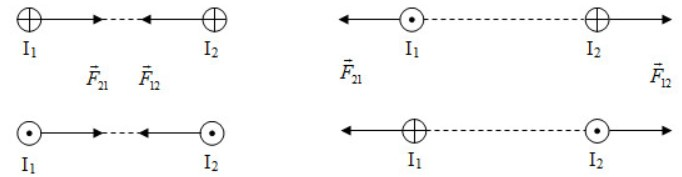
\includegraphics[scale=0.8]{../figs/VN11-PH-25-L-017-2-h102.jpg}
\end{center}
Hai dòng điện, cường độ tương ứng là $I_1$ và $I_2$ chạy trong hai dây dẫn thẳng dài, song song, cùng chiều thì hút nhau và ngược chiều thì đẩy nhau. 

Lực tương tác trên một độ dài $l$ của mỗi dây dẫn cho bởi:
	\begin{equation}
	F=2\cdot 10^{-7}\cdot \dfrac{I_1I_2}{r}\cdot l,
	\end{equation}
	trong đó,
	\begin{itemize}
		\item $I_1$ là cường độ của dòng điện qua dây dẫn thứ nhât. 
		\item $I_2$ là cường độ của dòng điện qua dây dẫn thứ hai. 
		\item $r$ là khoảng cách giữa hai dây dẫn.
		\item $l$ là chiều dài đoạn dây dẫn. 
	\end{itemize}
	
\subsection{Định nghĩa đơn vị ampe}

Ampe là cường độ của dòng điện không đổi khi chạy trong hai dây dẫn thẳng dài, song song, có tiết diện nhỏ, đặt cách nhau 1 m trong chân không, thì mỗi mét chiều dài của mỗi dây chịu tác dụng của một lực từ bằng $2\cdot 10^{-7}\ \text{N}$.

\section{Bài tập}
\begin{dang}{Lực tương tác giữa các dây dẫn thẳng dài đặt song song có dòng điện chạy qua}
\end{dang}

\textbf{Phương pháp giải}

Áp dụng kiến thức, các công thức về lực tương tác từ giữa hai dây dẫn thẳng, song song, có dòng điện chạy qua: 	$F=2\cdot 10^{-7}\cdot \dfrac{I_1I_2}{r}\cdot l$. 

Áp dụng quy tắc tổng hợp các vectơ lực trong trường hợp có nhiều dòng điện thẳng song song: $\vec{F}=\vec{F}_{1}+\vec{F}_{2}+...+\vec{F}_\text{n}$.



\luuy{Hai dòng điện cùng chiều thì hút nhau, hai dòng điện ngược chiều thì đẩy nhau}




\viduii{2}
{	
Dây dẫn thẳng dài thứ nhất có cường độ dòng điện là $I_1=5\ \text{A}$ đi qua đặt trong không khí. Tính lực từ dây thứ nhất tác dụng lên 3 m dây thứ hai có cường độ dòng điện là $I_2=10\ \text{A}$  đặt song song, cách dây thứ nhất 15 cm. Biết hai dòng điện ngược chiều.  


	\begin{mcq}(4)
		\item  $2\cdot 10^{-4}\ \text{N}$.
		\item  $2\cdot 10^{-5}\ \text{N}$.
		\item  $2\cdot 10^{-6}\ \text{N}$.
		\item  $2\cdot 10^{-7}\ \text{N}$.
	\end{mcq}
}{	
\begin{center}
		\textbf{Hướng dẫn giải:}
\end{center}
	
Lực từ dây thứ nhất tác dụng lên 3 m dây thứ hai là	$F=2\cdot 10^{-7}\cdot \dfrac{I_1I_2}{r}\cdot l=2\cdot 10^{-4}\ \text{N}$.

	
\textbf{	Đáp án: A.}
}

\viduii{2}{
	
Ba dây dẫn thẳng dài song song có khoảng cách $a=5\ \text{cm}$. Dây 1 và 3 được giữ cố định, có dòng $I_1=2I_3=4\ \text{A}$ đi qua như hình. Dây 2 tự do, có dòng $I_2=5\ \text{A}$ đi qua. Tìm chiều di chuyển của dây 2 và lực tác dụng lên 1 m dây 2 khi nó bắt đầu chuyển động nếu $I_2$ có chiều đi lên.

\begin{center}
	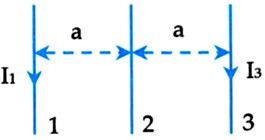
\includegraphics[scale=0.8]{../figs/VN11-PH-25-L-017-2-h101.jpg}
\end{center}
	\begin{mcq}
		\item Dây 2 di chuyển sang phải, $F_2=8\cdot 10^{-5}\ \text{N}$.
		\item Dây 2 di chuyển sang phải, $F_2=4\cdot 10^{-5}\ \text{N}$.
		\item Dây 2 di chuyển sang trái, $F_2=4\cdot 10^{-5}\ \text{N}$.
		\item Dây 2 di chuyển sang trái, $F_2=8\cdot 10^{-5}\ \text{N}$.
	\end{mcq}}
	{
\begin{center}
		\textbf{Hướng dẫn giải:}
\end{center}
	
	Lực từ do dây thứ nhất tác dụng do 1 m dây thứ hai là $F_{12}=2\cdot 10^{-7}\cdot \dfrac{I_1I_2}{r}\cdot l=8\cdot 10^{-5}\ \text{N}$.
	
	Lực từ do dây thứ ba tác dụng do 1 m dây thứ hai là $F_{32}=2\cdot 10^{-7}\cdot \dfrac{I_3I_2}{r}\cdot l=4\cdot 10^{-5}\ \text{N}$.
	
	Lực từ tổng hợp lên 1 m dây thứ hai: $\vec{F}_2=\vec{F}_{12}+\vec{F}_{32}$.
	
	Khi dòng điện thứ hai đi lên thì $\vec{F}_{12}$ ngược chiều $\vec{F}_{32}$.
	
	Suy ra,về độ lớn $F_2=\left| F_{12}-F_{32}\right|=4\cdot 10^{-5}\ \text{N}$.

  Do $F_{12}>F_{32}$ nên về chiều thì $\vec{F}_2$ sẽ cùng chiều $\vec{F}_{12}$.
  
  Vì vậy dây thứ 2 sẽ di chuyển sang phải.
	
\textbf{	Đáp án: B.}
	
}






